% Options for packages loaded elsewhere
\PassOptionsToPackage{unicode}{hyperref}
\PassOptionsToPackage{hyphens}{url}
%
\documentclass[
]{ltjsbook}
\usepackage{amsmath,amssymb}
\usepackage{lmodern}
\usepackage{iftex}
\ifPDFTeX
  \usepackage[T1]{fontenc}
  \usepackage[utf8]{inputenc}
  \usepackage{textcomp} % provide euro and other symbols
\else % if luatex or xetex
  \usepackage{unicode-math}
  \defaultfontfeatures{Scale=MatchLowercase}
  \defaultfontfeatures[\rmfamily]{Ligatures=TeX,Scale=1}
\fi
% Use upquote if available, for straight quotes in verbatim environments
\IfFileExists{upquote.sty}{\usepackage{upquote}}{}
\IfFileExists{microtype.sty}{% use microtype if available
  \usepackage[]{microtype}
  \UseMicrotypeSet[protrusion]{basicmath} % disable protrusion for tt fonts
}{}
\makeatletter
\@ifundefined{KOMAClassName}{% if non-KOMA class
  \IfFileExists{parskip.sty}{%
    \usepackage{parskip}
  }{% else
    \setlength{\parindent}{0pt}
    \setlength{\parskip}{6pt plus 2pt minus 1pt}}
}{% if KOMA class
  \KOMAoptions{parskip=half}}
\makeatother
\usepackage{xcolor}
\IfFileExists{xurl.sty}{\usepackage{xurl}}{} % add URL line breaks if available
\IfFileExists{bookmark.sty}{\usepackage{bookmark}}{\usepackage{hyperref}}
\hypersetup{
  pdftitle={統計力学の論理展開},
  pdfauthor={Sota Takahashi},
  hidelinks,
  pdfcreator={LaTeX via pandoc}}
\urlstyle{same} % disable monospaced font for URLs
\usepackage{graphicx}
\makeatletter
\def\maxwidth{\ifdim\Gin@nat@width>\linewidth\linewidth\else\Gin@nat@width\fi}
\def\maxheight{\ifdim\Gin@nat@height>\textheight\textheight\else\Gin@nat@height\fi}
\makeatother
% Scale images if necessary, so that they will not overflow the page
% margins by default, and it is still possible to overwrite the defaults
% using explicit options in \includegraphics[width, height, ...]{}
\setkeys{Gin}{width=\maxwidth,height=\maxheight,keepaspectratio}
% Set default figure placement to htbp
\makeatletter
\def\fps@figure{htbp}
\makeatother
\setlength{\emergencystretch}{3em} % prevent overfull lines
\providecommand{\tightlist}{%
  \setlength{\itemsep}{0pt}\setlength{\parskip}{0pt}}
\setcounter{secnumdepth}{-\maxdimen} % remove section numbering
\makeatletter
\@ifpackageloaded{subfig}{}{\usepackage{subfig}}
\@ifpackageloaded{caption}{}{\usepackage{caption}}
\captionsetup[subfloat]{margin=0.5em}
\AtBeginDocument{%
\renewcommand*\figurename{FIG.}
\renewcommand*\tablename{Table}
}
\AtBeginDocument{%
\renewcommand*\listfigurename{List of Figures}
\renewcommand*\listtablename{List of Tables}
}
\newcounter{pandoccrossref@subfigures@footnote@counter}
\newenvironment{pandoccrossrefsubfigures}{%
\setcounter{pandoccrossref@subfigures@footnote@counter}{0}
\begin{figure}\centering%
\gdef\global@pandoccrossref@subfigures@footnotes{}%
\DeclareRobustCommand{\footnote}[1]{\footnotemark%
\stepcounter{pandoccrossref@subfigures@footnote@counter}%
\ifx\global@pandoccrossref@subfigures@footnotes\empty%
\gdef\global@pandoccrossref@subfigures@footnotes{{##1}}%
\else%
\g@addto@macro\global@pandoccrossref@subfigures@footnotes{, {##1}}%
\fi}}%
{\end{figure}%
\addtocounter{footnote}{-\value{pandoccrossref@subfigures@footnote@counter}}
\@for\f:=\global@pandoccrossref@subfigures@footnotes\do{\stepcounter{footnote}\footnotetext{\f}}%
\gdef\global@pandoccrossref@subfigures@footnotes{}}
\@ifpackageloaded{float}{}{\usepackage{float}}
\floatstyle{ruled}
\@ifundefined{c@chapter}{\newfloat{codelisting}{h}{lop}}{\newfloat{codelisting}{h}{lop}[chapter]}
\floatname{codelisting}{Listing}
\newcommand*\listoflistings{\listof{codelisting}{List of Listings}}
\makeatother
\ifLuaTeX
  \usepackage{selnolig}  % disable illegal ligatures
\fi

\title{統計力学の論理展開}
\author{Sota Takahashi}
\date{}

\begin{document}
\maketitle

{
\setcounter{tocdepth}{3}
\tableofcontents
}
\hypertarget{ux5b64ux7acbux3057ux305fux5358ux7d14ux306aux53e4ux5178ux7cfbux306eux7d71ux8a08ux529bux5b66}{%
\section{孤立した単純な古典系の統計力学}\label{ux5b64ux7acbux3057ux305fux5358ux7d14ux306aux53e4ux5178ux7cfbux306eux7d71ux8a08ux529bux5b66}}

\hypertarget{ux7b49ux91cdux7387ux306eux539fux7406}{%
\subsection{等重率の原理}\label{ux7b49ux91cdux7387ux306eux539fux7406}}

古典系の統計力学では、以下の2つを念頭に置く。

\begin{description}
\tightlist
\item[\textbf{ミクロな状態}]
その系の(途方も無い)自由度のぶんだけの一般化運動量と一般化座標の次元をもつ\textbf{相空間}があれば、その上の1点は必ず系のひとつのミクロ状態を記述している。
\item[\textbf{マクロな状態}]
エントロピーとその自然な変数で張られる(ミクロ系よりは)ごく少ない自由度の\textbf{相空間}上の一点を使ってその系の平衡状態を指定できる
\end{description}

\begin{figure}
\hypertarget{fig:micro_macro}{%
\centering
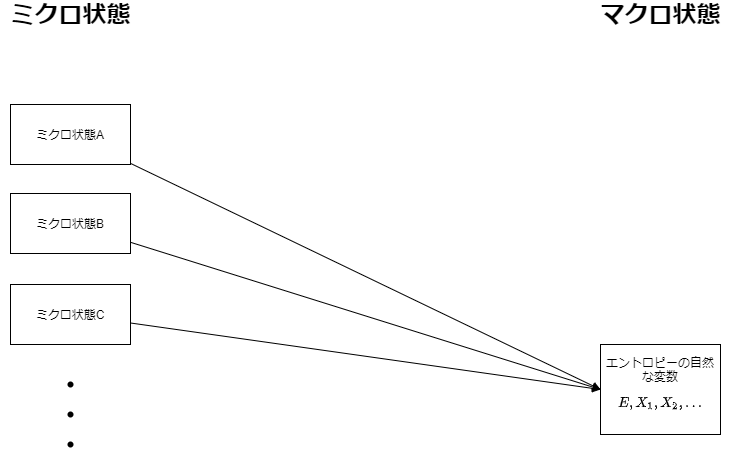
\includegraphics{images/micro_macro.drawio.png}
\caption{マクロ変数を使って対応するミクロ状態を指定する。ミクロ状態には膨大な数があり、平衡状態であり続けるというマクロな状況が続く限り、ミクロ状態はマクロ状態が許す総エネルギーなどの拘束のもとでのみ変化する。}\label{fig:micro_macro}
}
\end{figure}

FIG.~\ref{fig:micro_macro}のマクロ状態で指定した状態が平衡状態の場合、左側の「ミクロ状態」から任意のものを一つ選び出してきたとき、取り出された状態の\textbf{ほぼ全て}が区別できず、同じ平衡状態に対応するとしよう。これは統計力学の要請のもっとも基本的なものの一つである。

この操作で選び出す母集団となったミクロ状態たちを\textbf{ミクロカノニカル集団}とよぶ。

ここでいう\textbf{ほぼ全て}は、以下の極限で確率100\%になるとする。

\begin{description}
\tightlist
\item[熱力学極限]
エントロピーの自然な変数の\textbf{密度}を一定にしながら、体積をあらゆる方向に一樣に大きくしていって無限大にする極限のこと
\end{description}

ミクロカノニカル集団の要素それぞれの実現確率を等しく与えた確率分布のことを\textbf{ミクロカノニカル分布}とよぶ。先ほどの要請と合わせると、ミクロカノニカル分布は平衡状態とマクロにみて同じ状態を実現する。

これを等重率の原理として採用する。 これによれば、

\begin{itemize}
\tightlist
\item
  マクロな変化がない限り、平衡状態は平衡状態のままである
\item
  殆どの場合、孤立した単純系は平衡状態にやがて落ち着く
\end{itemize}

というマクロな観測は以下のように説明される。

「ミクロな状態は平衡状態でも時間発展している。その時間発展とはミクロカノニカル集団のうちのある要素から別の要素に移ることにほかならないが、非平衡状態からそれを繰り返せば圧倒的大多数であるところの平衡状態にたどり着く。十分マクロな系では、一度平衡状態になったときに次の状態が非平衡状態になる確率はゼロである。」

非常に普遍的な事実をこのように自然な形で説明できるというのがこの原理を採用する理論のよいところである。
等重率の「原理」は自然界が厳密に従う原理というわけではなく、理論で公理的に採用して自然現象を理解しようという意味での原理である。そして、仮説であるところのこの公理からマクロな物理量を計算したときに、確率的なゆらぎが小さければ検証が可能である。

\hypertarget{ux30a8ux30f3ux30c8ux30edux30d4ux30fcux3092ux30dfux30afux30edux306aux8996ux70b9ux304bux3089ux8a08ux7b97ux3067ux304dux308bux304b}{%
\subsection{エントロピーをミクロな視点から計算できるか?}\label{ux30a8ux30f3ux30c8ux30edux30d4ux30fcux3092ux30dfux30afux30edux306aux8996ux70b9ux304bux3089ux8a08ux7b97ux3067ux304dux308bux304b}}

熱力学は、ミクロな物理量から直接には定めることができない、\textbf{純熱力学変数}が含まれている。
等重率の原理は、ミクロな物理量がマクロな物理量として現れてくるときに平均が使えることを教えてくれるから、力学変数についてはマクロなスケールでも知ることができる。
ここでは純熱力学変数をマクロな物理学に整合するように、等重率の原理とミクロな物理学を用いてエントロピーを求める方法がないか推測する。
もし正しく求められるものがあれば、それを要請として統計力学を構築すれば良い。

等重率の原理が教えてくれるのはミクロなエネルギーの分布であるから、エネルギーとエントロピーとの関係を考えてみよう。
熱力学から得られる知見として、

\begin{quote}
熱の交換が可能な2つの単純系からなる複合系が平衡状態に達しているとき、
それらの単純系のエントロピーのエネルギーに共役な示強変数(\textbf{逆温度})の値は一致する
\end{quote}

というものがある。 すなわち、

\begin{equation}\protect\hypertarget{eq:inverse-temperature}{}{
\frac{\partial}{\partial E^{(1)}}S^{(1)}(E^{(1)})=\frac{\partial}{\partial E^{(2)}}S^{(2)}(E^{(2)})
}\label{eq:inverse-temperature}\end{equation} である。
平衡状態についての記述は別にエネルギーに共役な物に限らずあらゆる示強変数について言えるだろうが、
以下では等重率の原理が直接に決めるエネルギーに関する平衡条件だけを考えるので、逆温度についてのこの関係を使っていこう。

ここでミクロカノニカル分布をしているのは単純系に限っていたことに気づく。
では逆に考えて、単純系を全く無意味な壁で区切って部分系(1)と部分系(2)からなる複合系とみなせば良いのである。
そうすれば、単純系の中で逆温度の等式が利用できる。

部分系がそれぞれ十分に大きく、先程の「無意味な壁」のあたりで起きる系間の相互作用が無視できるほどであれば、それぞれの部分系が孤立しているときの状態数の積で全系の状態数が表せるはずだ。
すなわち、エネルギーEのときのミクロカノニカル分布で与えられる系の状態数を\(W(E)\)で表して
\[
W(E)=\sum_{E^{(1)}}W^{(1)}(E^{(1)})W^{(2)}(E-E^{(1)})
\]

この関係式は、粒子間の相互作用には短距離力しか効かない(長距離秩序がない?)という仮定のもとでよく成り立つと期待されるが、
厳密に成り立っているかどうかよりもこれを使って熱力学的要請を満たすエントロピーを表現できるかどうかが肝である。
等重率の原理によれば、\(W(E)\)が特定の値\(E^{(1)}\)を持っている確率\(\Theta^{(1)}(E^{(1)})\)は
\begin{equation}\protect\hypertarget{eq:E1probability}{}{
\Theta^{(1)}(E^{(1)}) = \frac{W^{(1)}(E^{(1)})W^{(2)}(E-E^{(1)})}{W(E)}
}\label{eq:E1probability}\end{equation} である。

所与の物理量を満たす状態のうちでもっともありふれた状態が平衡状態である、ということは逆に、
確率が最も高い状態を作り出す物理量がその物理量の平衡値である、といえる。
したがって、eq.~\ref{eq:E1probability}において与えられた\(E\)のもとで\(\Theta^{(1)}(E^{(1)})\)、\(\Theta^{(2)}(E^{(2)})\)をともに最大にするような\(E_1, E_2\)を求めると、この複合系のエネルギーの平衡値が求められることになる。

関数の最大値は微分によって求められるのだから、
\begin{equation}\protect\hypertarget{eq:equilibrium-value-of-E}{}{
\frac{\partial}{\partial E^{(1)}}\ln{W^{(1)}}(E^{(1)})=\frac{\partial}{\partial E^{(2)}}\ln{W^{(2)}}(E^{(2)})
}\label{eq:equilibrium-value-of-E}\end{equation}
を計算すればよい。ここで、 \[
\frac{\partial}{\partial E^{(1)}}\ln{W^{(2)}}(E-E^{(1)})=-\frac{\partial}{\partial E^{(2)}}\ln{W^{(2)}}(E^{(2)})
\] を用いた(合成関数の微分と連鎖律)。

eq.~\ref{eq:equilibrium-value-of-E}を熱力学からきたeq.~\ref{eq:inverse-temperature}と比較すれば、統計力学のエントロピーが満たすべき性質が見えてくる。
まずざっくりと\(\ln{W}\)と\(S\)が対応していることはみればわかる。微分の形で対応しているということは、定数倍と定数和だけの自由度があってよく、
\[
S^{(i)} = (定数A)\times\ln W^{(i)}+(定数B)\quad(i=1, 2)
\]
のような関係性のはずだ。定数Bはエントロピーの原点をどこにとるか、という話だから、ゼロに選ぶのが自然だろう。定数Aには、単位系を熱力学に合わせるべく、
\[
k_B\approxeq1.38\times10^{-23} \text{J/K}
\]
とする。これを\textbf{ボルツマン定数}と呼ぶ。理論物理では\(k_B=1\)として単位系を構成することもある。
ここまでで、分割した系の独立性や平衡値が\(E^{(1)}\)、\(E^{(2)}\)とゆらぎが十分小さいとみなせる範囲で決まることなど、
十分系のサイズが大きいということを前提とした等式を利用してきたことに注意して、任意の単純系に拡張して書くと、

\begin{description}
\tightlist
\item[ボルツマンの定理]
エントロピーの自然な変数\(E, X_1, \cdots, X_t\)と書ける単純系では\(V\to\infty\)で熱力学のエントロピーに漸近する量
\[
S(E, X_1, \cdots, X_t) = k_B\ln{W(E, X_1, \cdots X_t)}+o(V)
\] がある。
\end{description}

ここでオーダーの記号\(o(V)\)は、\(V\to\infty\)という極限で\(0\)になる項であることを表す。

\end{document}
